%----------------------------------------------------------------------------------------
%	PAKET-/ UND ANDERE DOKUMENT-IMPORTS
%----------------------------------------------------------------------------------------
\documentclass{scrartcl}   % Formateinstellungen
\usepackage[ngerman]{babel} % deutsche Silbentrennung
\usepackage[utf8]{inputenc} % deutsche Umlaute
\usepackage{placeins}   % verbessert Anzeige eines Floats hinter dem Befehl \FloatBarrier
\usepackage{amsfonts}   % neue Schriftanpassungen (wird von amssymb (s.u.) geladen)
\usepackage{amssymb}    % erweitert Benutzung von amsfonts (s.o.)
\usepackage{amsmath}    % Vielzahl von neuen mathematischen Umgebungen und Befehlen (wird von mathtools (s.u.) geladen)
\usepackage{mathtools}  % Verbesserung von amsmath (s.o.)
\usepackage{booktabs}   % Tabellen ohne vertikale Striche
\usepackage{siunitx}    % Einheitensystem
\usepackage[margin={0.3cm,0.3cm},font=singlespacing,labelfont=bf,labelsep=endash]{caption} % Bildunterschriften
\usepackage{wrapfig}    % Bild von Text umfließen lassen
\usepackage{sidecap}    % ermöglicht Überschriften neben Bildern / Tabellen
\usepackage{setspace}   % zum Definieren des Zeilenabstandes
\usepackage{eurosym}    % ergänzt optimales Euro-Zeichen
\usepackage[perpage,marginal]{footmisc} % ermöglicht Fußnoten und das Verändern dieser
\usepackage{graphicx}   % ermöglicht besseres Einbinden von Grafiken
\usepackage{fancyhdr}   % zum Erstellen von Kopf- und Fußzeilen
\usepackage{listings}   % ermöglicht Quellcodelisting
\usepackage{color}  % Farb-Management von Vorder- und Hintergrundfarben
\usepackage{pdfpages}   % ermöglicht das Einbinden von ganzen oder nur Teilen von PDFs
\usepackage{lineno} % Zeilenzählung
\usepackage{framed} % ermöglicht das Einrahmen von Elementen
\usepackage{pifont} % fügt Symbol-Schriften hinzu
\usepackage[hidelinks]{hyperref}    % ermöglicht das Hinzufügen von Links und Verweisen innerhalb
                                    % des PDF Dokuments und weitere Einstellungen
\usepackage[left=2.5cm,right=2cm,top=2cm,bottom=2cm,includeheadfoot]{geometry}  % Größenanpassung der Seite
%----------------------------------------------------------------------------------------


%----------------------------------------------------------------------------------------
%   KONFIGURATIONEN
%----------------------------------------------------------------------------------------
\begin{document}
\setlength{\parskip}{1ex}   % Abstand zwischen Absätzen 
\parindent 0pt  % legt Einrücke der ersten Zeile fest
\renewcommand{\thefigure}{\arabic{figure}.\alph{ab}}    % Umdefinieren von Bildnummern

\definecolor{darkblue}{rgb}{0,0,.6} % Festlegen der Farben
\definecolor{darkred}{rgb}{.6,0,0}  % Festlegen der Farben
\definecolor{darkgreen}{rgb}{0,.6,0}    % Festlegen der Farben
\definecolor{red}{rgb}{.98,0,0} % Festlegen der Farben
\definecolor{purple}{rgb}{0.44, 0.16, 0.39}  % Festlegen der Farben

\lstloadlanguages{Java} % lädt Programmiersprachen
\lstset{language=Java,basicstyle=\footnotesize\ttfamily,commentstyle=\itshape\color{darkgreen},keywordstyle=\bfseries\color{darkblue},stringstyle=\color{darkred},tabsize=3,showspaces=false,showtabs=false,columns=fixed,numbers=left,frame=single,numberstyle=\tiny,breaklines=true,showstringspaces=false,xleftmargin=1cm} % Erstellen eines Codeblocks
    
\pagestyle{fancy}   % Setzen des Seitenstyles "fancy" ermöglicht eigenes Erstellen einer Kopf- und Fußzeile
\fancyhf{}  % alle Kopf- und Fußzeilenfelder bereinigen
\fancyhead[L]{\leftmark}    % Kopfzeile links (mit "leftmark" erstellt man im Header das Chapter, mit "rightmark" die Section)
\fancyhead[C]{} % zentrierte Kopfzeile
\fancyhead[R]{\thepage} % Kopfzeile rechts
\fancypagestyle{plain}  % legt Seiten-Typen fest

\newcommand{\barrow}{\item[\ding{228}]} % hinzufügen des Pfeil-Aufzählsymbols unter dem Command \barrow
%----------------------------------------------------------------------------------------


%----------------------------------------------------------------------------------------
%   1. SEITE
%----------------------------------------------------------------------------------------
\titlehead{\Large

\begin{center}
\begin{framed}
\centering {Inoffizielle Lösungen und Erklärungen - \href{https://www.inf-schule.de/inf-schule}{inf-schule\textsuperscript{\textcopyright}} (\href{https://creativecommons.org/licenses/by-sa/4.0/legalcode.de}{\textit{Lizenz}})}

\centering {\Large\textbf{\href{https://inf-schule.de/programmierung/oopjava}{2.3 Objektorientierte Programmierung mit Java}}}
\end{framed}
\end{center}}

\title{\huge{\href{https://www.inf-schule.de/programmierung/oopjava/implementierung/frog}{2.3\\Frog}}\\
\vspace{0.5cm}
\begin{figure}[ht]
	\centering
	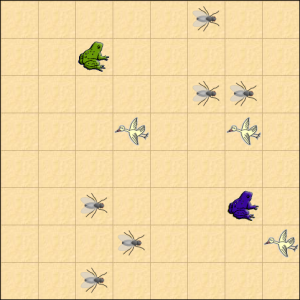
\includegraphics[height=4.5cm]{Frog.png}
\end{figure}
\vspace{2cm}}

\author{\textbf{Benötigte IDEs:}\\
\href{https://www.greenfoot.org/}{Greenfoot}, \href{https://www.bluej.org/}{BlueJ}
\vspace{2cm}}

\date{\textbf{Verfasser:}\\
\href{https://nikothegreek.jimdofree.com/}{Niko Diamadis}\\
\vspace{0.5cm}
\textbf{Erstellungs-/ Änderungsdatum}\\
\today\enlargethispage{4cm}}
%----------------------------------------------------------------------------------------

%----------------------------------------------------------------------------------------
%   2. SEITE
%----------------------------------------------------------------------------------------
\doublespacing

\maketitle\thispagestyle{empty}

\numberwithin{equation}{section}
\cleardoublepage

\setcounter{page}{1}
\tableofcontents
%----------------------------------------------------------------------------------------


%----------------------------------------------------------------------------------------
%   3. UND NACHFOLGENDE SEITEN
%----------------------------------------------------------------------------------------
\newpage
\pagenumbering{arabic}  % Ändern der Seitenangabe

\cleardoublepage

\section{Spielidee}

Zu dieser Seite sind meines Erachtens nach keine Anleitungen und/oder Erläuterungen nötig.\\
Wenn doch Fragen aufkommen, schreib' einfach an \textbf{\href{mailto:nikodiamond3@gmail.com}{nikodiamond3@gmail.com}}.

\newpage

\section{Implementierung}

\subsection{Vorlage öffnen}

Der gewünschte Effekt tritt nicht ein, da zwar abgefragt wird, welches Bild das zu erzeugende Objekt erhalten soll, jedoch wird dem Objekt noch kein Bild zugewiesen, sodass das Objekt das Standardbild (einen Greenfoot-Fuß) erhält.

\subsection{Aufbau der Dokumentation}

Beim Öffnen der Dokumentation landet man auf der Übersicht aller Klassen inklusive Beschreibung dieser.\\
Wenn man nun auf eine der Klassen klickt, kommt man auf eine klasseneigene Seite. Dort stehen oben eine Beschreibung, wofür diese Klasse benutzt wird, und weitere Informationen zur Nutzung der Klasse.

Weiter unten findet man anschließend mögliche Konstruktoren, teilweise auch hier mit Beschreibung.

Noch weiter unten sind alle Methoden mit Signatur und Beschreibung aufgelistet. Einige der Methoden werden unter der Tabelle weiter beschrieben und erklärt, wie sie zu benutzen sind.

\subsection{Methoden finden}

\begin{itemize}
    \barrow \textcolor{darkred}{void} \textbf{setImage}(\textit{Greenfoot Image}) - Actor
    \barrow \textcolor{darkred}{int} \textbf{getX()} - Actor\\
    \textcolor{darkred}{int} \textbf{getY}() - Actor
    \barrow \textcolor{darkred}{void} \textbf{setLocation}(\textit{int x, int y}) - Actor
    \barrow \textcolor{darkred}{void} \textbf{addObject}(\textit{Actor object, int x, int y}) - World
    \barrow \textcolor{darkred}{int} \textbf{getWidth}() - World
    \barrow \textcolor{purple}{static} \textcolor{darkred}{int} \textbf{getRandomNumber}(int limit) - Greenfoot
    \barrow \textcolor{purple}{static} \textcolor{darkred}{void} \textbf{stop}() - Greenfoot
\end{itemize}

\newpage

\subsection{Basisfunktionalität}

\begin{itemize}
    \barrow Setzen des Bildes:\\
    \begin{lstlisting}
public Frosch(String startbild) {
    kraft = 20;
    setImage(startbild);
}
    \end{lstlisting}
    \barrow Erzeugen eines grünes und eines blaues Frosch am Anfang (die Größe der Frosch-Welt ist im Konstruktor abzulesen, sie ist 8 x 8 Felder groß):\\
    \begin{lstlisting}
public FrogWorld() {    
    super(8, 8, 60);
    
    int x = Greenfoot.getRandomNumber(getWidth());
    int y = Greenfoot.getRandomNumber(getHeight());
    
    addObject(new Frosch("froschgruen.png"), x, y);
    
    x = Greenfoot.getRandomNumber(getWidth());
    y = Greenfoot.getRandomNumber(getHeight());
    
    addObject(new Frosch("froschblau.png"), x, y);
}
    \end{lstlisting}
    
    Damit die Zeilen wieder nicht zu lang werden, habe ich hier wieder lokale Variablen benutzt.
\end{itemize}

\newpage

\subsection{Springen}

Zum Lösen benutze ich den schon gegebenen Lösungsansatz.\\
\begin{lstlisting}
public void act() {
    ...
    kraft--;
}

public void springen() {
    int xDiff = Greenfoot.getRandomNumber(3) - 1;
    int yDiff = Greenfoot.getRandomNumber(3) - 1;
    
    setLocation(getX() + xDiff, getY() + yDiff);
}
\end{lstlisting}

\subsection{Fliegen würfeln}

\begin{itemize}
    \barrow
    \begin{itemize}
        \item \textbf{1. Zeile}\\
        Bedingung, welche erfüllt ist, wenn eine bei jeder Wiederholung neu erstellte Zufallszahl kleiner 5 ist. Solange sie erfüllt ist, wird der Code in den geschweiften Klammern immer wieder wiederholt.
        \item \textbf{2. Zeile}\\
        Die lokale Variable \texttt{x} wird erstellt und zufällig mit einem Wert maximal so groß wie die Breite der Welt belegt.
        \item \textbf{3. Zeile}\\
        Die lokale Variable \texttt{y} wird erstellt und zufällig mit einem Wert maximal so groß wie die Höhe der Welt belegt.
        \item \textbf{4. Zeile}\\
        Ein neues Objekt wird in der Welt an die Stelle (\texttt{x}|\texttt{y}) gesetzt.
    \end{itemize}
    \barrow Damit es weniger Störche gibt als Fliegen, habe ich die Warscheinlichkeit, dass die Bedingung in der zweiten Schleife erfüllt ist, herabgesetzt.\\
    Außerdem benutze ich \texttt{x} und \texttt{y} wieder, da man die Koordinaten der beiden Frösche nicht mehr braucht.\\
    \begin{lstlisting}
while (Greenfoot.getRandomNumber(6) < 5) {
    x = Greenfoot.getRandomNumber(getWidth());
    y = Greenfoot.getRandomNumber(getHeight());
    addObject(new Fliege(), x, y);
}
    
while (Greenfoot.getRandomNumber(6) < 3) {
    x = Greenfoot.getRandomNumber(getWidth());
    y = Greenfoot.getRandomNumber(getHeight());
    addObject(new Storch(), x, y);
}
    \end{lstlisting}
\end{itemize}

\subsection{Fliegen fester Anzahl}

Auch hier habe ich das Beispiel verwirklicht.\\
\begin{lstlisting}
int i = 0;
        
while (i < 5) {
    x = Greenfoot.getRandomNumber(getWidth());
    y = Greenfoot.getRandomNumber(getHeight());
    addObject(new Fliege(), x, y);
    
    i++;
}

i = 0;



while (i < 3) {
    x = Greenfoot.getRandomNumber(getWidth());
    y = Greenfoot.getRandomNumber(getHeight());
    addObject(new Storch(), x, y);
    
    i++;
}
\end{lstlisting}

\subsection{Fliegen zufälliger Anzahl}

Auch hier habe ich das Beispiel verwirklicht.\\
\begin{lstlisting}
while (i < Greenfoot.getRandomNumber(5) + 4) {
    //Fliegen
    ...
}

...

while (i < Greenfoot.getRandomNumber(4) + 2) {
    //Stoerche
    ...
}
\end{lstlisting}

\subsection{Transparenz}

\begin{lstlisting}
public void act() {
    if (kraft <= 0) {
        getImage().setTransparency(128);
        Greenfoot.stop();
    }

    ...
}
\end{lstlisting}

Um etwas halbtransparent darzustellen, habe ich als Transparenz-Wert gerundet die Hälfte des maximalen Wertes (welcher in der Dokumentation zu finden ist) benutzt, nämlich 128.

\subsection{Essen}

\begin{lstlisting}
public void essen() {
    if (isTouching(Fliege.class)) {
        kraft += 10;
        removeTouching(Fliege.class);
    }
}
\end{lstlisting}

\subsection{Treffe Storch}

\begin{lstlisting}
public void treffeStorch() {
    if (isTouching(Storch.class)) {
        Greenfoot.stop();
        getImage().setTransparency(128);
    }
}
\end{lstlisting}

\newpage

\subsection{for-Schleifen}

Der in \hyperlink{subsection.2.7}{\textbf{2.7}} und \hyperlink{subsection.2.8}{\textbf{2.8}} aufgezeigte Code kann durch folgenden Code mit for-Schleifen ersetzt werden:\\
\begin{lstlisting}
for (int i = 0; i < Greenfoot.getRandomNumber(5) + 4; i++) {
    x = Greenfoot.getRandomNumber(getWidth());
    y = Greenfoot.getRandomNumber(getHeight());
    addObject(new Fliege(), x, y);
}
        
for (int i = 0; i < Greenfoot.getRandomNumber(4) + 2; i++) {
    x = Greenfoot.getRandomNumber(getWidth());
    y = Greenfoot.getRandomNumber(getHeight());
    addObject(new Storch(), x, y);
}
\end{lstlisting}

\newpage

\section{Fachkonzept - Klassendokumentation}

Zu dieser Seite sind meines Erachtens nach keine Anleitungen und/oder Erläuterungen nötig.\\
Wenn doch Fragen aufkommen, schreib' einfach an \textbf{\href{mailto:nikodiamond3@gmail.com}{nikodiamond3@gmail.com}}.

\newpage

\section{Fachkonzept - Klassen und primitive Datentypen}

Zu dieser Seite sind meines Erachtens nach keine Anleitungen und/oder Erläuterungen nötig.\\
Wenn doch Fragen aufkommen, schreib' einfach an \textbf{\href{mailto:nikodiamond3@gmail.com}{nikodiamond3@gmail.com}}.

\newpage

\section{Fachkonzept - Wiederholungen}

Zu dieser Seite sind meines Erachtens nach keine Anleitungen und/oder Erläuterungen nötig.\\
Wenn doch Fragen aufkommen, schreib' einfach an \textbf{\href{mailto:nikodiamond3@gmail.com}{nikodiamond3@gmail.com}}.

\newpage

\section{Übungen}

\subsection{Greenfoot-Klassen}

\begin{figure}[ht]
    \centering
	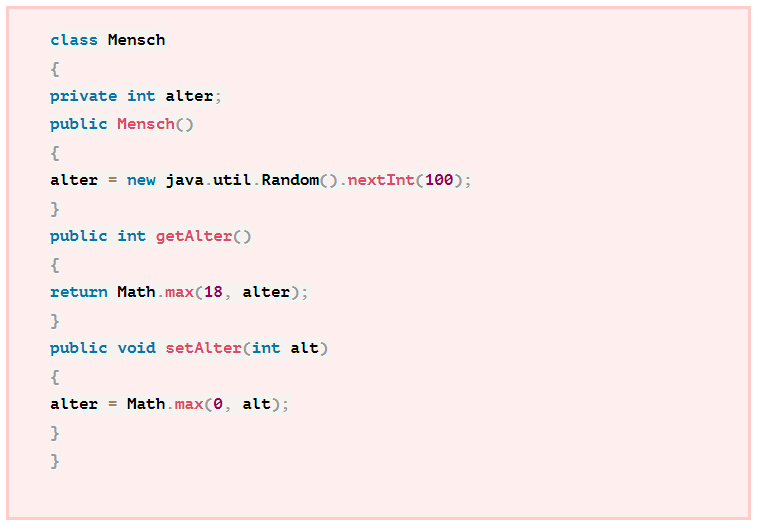
\includegraphics[height=15cm]{2.3.2.3/6.Uebungen/1-1.png}
\end{figure}

\newpage

\subsection{Frog erweitern}

\begin{itemize}
    \item[\textbf{1.}] Zuerst muss die Datei im Projektordner in den Ordner \glqq sounds\grqq{} abgelegt werden.\\
    \begin{lstlisting}
public FrogWorld() {    
    ...
    
    new GreenfootSound("frosch.mp3").play();
}
    \end{lstlisting}
    \item[\textbf{2.}] Mit den Parametern muss man ein bisschen herumprobieren, irgendwann kommt man auf angemesse Ergebnisse.\\
    \begin{lstlisting}
public void act() {
    if (kraft <= 0) {
        ...
        getImage().scale(35, 35);
        ...
    }

public void treffeStorch() {
    if (isTouching(Storch.class)) {
        ...
        getImage().scale(35, 35);
    }
}
    \end{lstlisting}
    \item[\textbf{3.}] Es soll also nur bei Berührung mit einer Fliege und nur wenn sie nicht halbtransparent ist die Kraft erhöht werden. Logischerweise wird bei Berührung die Fliege halbtransparent dargestellt (nicht verwirren lassen von den if-Bedingungen, sie sind zu lang für eine Zeile, deshalb wurden Zeilensprünge benutzt; beim Programmieren einfach Zeilensprünge wegdenken).
    
    \newpage
    
    \begin{lstlisting}
public void essen() {
    if (isTouching(Fliege.class) && getOneIntersectingObject(Fliege.class).getImage().getTransparency() != 128) {
        kraft += 10;
        getOneIntersectingObject(Fliege.class).getImage().setTransparency(128);
    }
}
    \end{lstlisting}
    \item[\textbf{4.}] Ich habe mich für die Variante entschieden, in der man den Strings des ersten Bildes speichert. Diesen rufe ich jeden \texttt{act}-Schritt neu aus, um die vorherige Zahl auf dem Bild nicht einfach mit der neuen zu \glqq überdrucken\grqq{}.\\
    Außerdem muss man in der if-Schleife am Ende ein \texttt{return} ergänzen (so bricht man die Methode vorzeitig ab), damit die Transparenz und das skalierte Bild nicht am Ende wieder durch das Anfangsbild ersetzt werden und eine \texttt{-1} statt der erwünschten 0 erscheint (Falls du es nicht verstehst, teste einfach was passiert, wenn man es weglässt).\\
    \begin{lstlisting}
String img;

public void act() {
    if (kraft <= 0) {
        ...
        return;
    }

    ...

    kraft--;
    
    setImage(img);
    getImage().drawString(kraft + "", 5, 10);
}
    \end{lstlisting}
    Die beiden letzten Parameter der \texttt{drawString}-Methode beschreiben die Position der Schrift auf dem Bild, hier habe ich einfach ein bisschen herumprobiert, bis sie ganz gut gepasst hat (und zwar oben links über den Fröschen).
    
    \item[\textbf{5.}] Diese Aufgabe ist schon etwas komplizierter. Angefangen habe ich mit dem Implementieren eines neuen Actors zum mehrfachen Zugreifen auf die getroffene Fliege, da ich auch noch darauf zugreifen können muss, wenn der Frosch sie nicht mehr berührt.
    
    Wenn ein Frosch nun also eine noch lebendige Fliege berührt, wird dem neuen Actor diese Fliege zugewiesen, zudem wird sie halbtransparent dargestellt und die \texttt{10} erscheint (diesmal oben rechts).
    
    Um nun nach einer bestimmten Anzahl von \texttt{act}-Schritten die \texttt{10} wieder zu entfernen, brauchen wir eine Zählvariable, welche in jedem \texttt{act}-Schritt erhöht wird (bei mir heißt sie \texttt{timer}).
    
    Der nächste Schritt ist dann zu erkennen, ob der Timer eine bestimmte Zahl erreicht hat. Da \texttt{timer} mit dem Wert \texttt{0} initialisiert wird und jeder positive Wert durch das durchgehende Ausführen der \texttt{act}-Methode ohne Berührung einer Fliege erreicht werden kann und eine Bedingung, welche z.B. auf den Wert \texttt{5} wartet, in dem Fall dann sinnlos wäre, setze ich \texttt{timer} beim Essen einer Fliege auf \texttt{-6}, damit ich bei Wert \texttt{-1} mithilfe einer einfachen if-Schleife die \texttt{10} wieder entfernen kann. \texttt{-1} kann nämlich nur erreicht werden, wenn \texttt{timer} vorher auf unter \texttt{0} gesetzt wird (bei uns in der \texttt{essen}-Methode).
    
    Dadurch bleibt die \texttt{10} 5 \texttt{act}-Schritte lang stehen, bis sie dann wieder entfernt wird. Jedoch muss man auch beachten, dass währenddessen auch eine andere Fliege berührt werden kann.\\
    Dafür überprüfe ich am Anfang der \texttt{essen}-Methode noch, ob dem Actor \texttt{tote\_fliege} schon eine Fliege zugewiesen ist, wo gerade \texttt{10} steht. Wenn der Actor also nicht den Wert \texttt{null} hat, wird der Wartevorgang vorzeitig abgebrochen, bei der älteren toten Fliege wird die \texttt{10} entfernt und der Vorgang beginnt mit der neuen toten Fliege.\\
    
    \newpage
    
    \begin{lstlisting}
Actor tote_fliege;
int timer;

public void act() {
    ...
    
    timer++;
}
    
public void essen() {
    if (isTouching(Fliege.class) && getOneIntersectingObject(Fliege.class).getImage().getTransparency() != 128) {
        if (tote_fliege != null) {
            tote_fliege.setImage("fly.png");
        }
        
        tote_fliege = getOneIntersectingObject(Fliege.class);
        tote_fliege.getImage().setTransparency(128);
        tote_fliege.getImage().drawString("10", 30, 10);
        
        kraft += 10;
        timer = -6;
    }
    
    if (timer == -1) {
        tote_fliege.setImage("fly.png");
        tote_fliege.getImage().setTransparency(128);
        tote_fliege = null;
    }
}
    \end{lstlisting}
    \item[\textbf{6.}] Bei dieser Aufgabe habe ich folgenden Lösungsansatz:\\
    Ich erstelle durch die schon bestehenden for-Schleifen die Fliegen und Störche, lasse jedoch jedes dieser Objekte aus ihrer eigenen Klasse heraus überprüfen, ob sie noch ein anderes Objekt berühren (mithilfe einer Methode, die ich in \texttt{World} aufrufe).
    
    In der Fliegen-for-Schleife erstelle ich also eine neue Fliege, welche ich an eine zufällige Position setze und dann die Methode \texttt{check} an der Fliege aufrufe. Diese Methode setzt die Fliege solange an eine zufällige Position, bis sie keine andere mehr berührt (Störche müssen noch nicht beachtet werden, es gibt nämlich noch keine).
    
    Anschließend passiert dasselbe mit den Störchen, nur mit dem Unterschied, dass die while-Schleife solange ausgeführt wird, bis weder ein Storch noch eine Fliege berührt wird.\\
    \begin{lstlisting}
public FrogWorld() {    
    ...
    
    for (int i = 0; i < Greenfoot.getRandomNumber(5) + 4; i++) {
        Fliege fliege = new Fliege();
        int x = Greenfoot.getRandomNumber(getWidth());
        int y = Greenfoot.getRandomNumber(getHeight());
        addObject(fliege, x, y);
        fliege.check();
    }
    
    for (int i = 0; i < Greenfoot.getRandomNumber(4) + 2; i++) {
        Storch storch = new Storch();
        int x = Greenfoot.getRandomNumber(getWidth());
        int y = Greenfoot.getRandomNumber(getHeight());
        addObject(storch, x, y);
        storch.check();
    }
    
    ...
}
    \end{lstlisting}
    
    \newpage
    
    \begin{lstlisting}
//Fliege
void check() {
    while (isTouching(Fliege.class)) {
        int x = Greenfoot.getRandomNumber(getWorld().getWidth());
        int y = Greenfoot.getRandomNumber(getWorld().getHeight());
        
        setLocation(x, y);
    }
}
    \end{lstlisting}
    \begin{lstlisting}
//Storch
void check() {
    while (isTouching(Storch.class) || isTouching(Fliege.class)) {
        int x = Greenfoot.getRandomNumber(getWorld().getWidth());
        int y = Greenfoot.getRandomNumber(getWorld().getHeight());
        
        setLocation(x, y);
    }
}
    \end{lstlisting}
\end{itemize}

\subsection{Anzeige auf der Welt}

Nur die zweite Variante funktioniert, da nur ein Objekt aus der Unterklasse zum Objekt aus der oberen Klasse konvertiert werden, andersherum funktioniert es nicht (\glqq Ein Schüler ist ein Mensch, aber ein Mensch ist nicht unbedingt ein Schüler.\grqq)

\newpage

\subsection{Java Klassenbibliothek}

Der hier gezeigte Code muss in keine Klasse geschrieben werden, sondern kann ins Codepad (die Direkteingabe) eingegeben werden. Deshalb muss man sich nochmal ins Gedächtnis rufen, dass bei Rückgabe eines Wertes kein Semikolon gesetzt wird, ansonsten wird kein Wert ausgegeben.

Teste es am besten auch mal selber.

\begin{itemize}
    \barrow Zuerst muss man in der Dokumentation in der String-Klasse die richtige Methode finden. Danach erstellt man irgendeinen String und ruft an diesem die Methode \texttt{length} ohne Parameter auf, als Rückgabe bekommt man die Länge des Strings.
    
    \begin{figure}[ht]
	    \centering
	    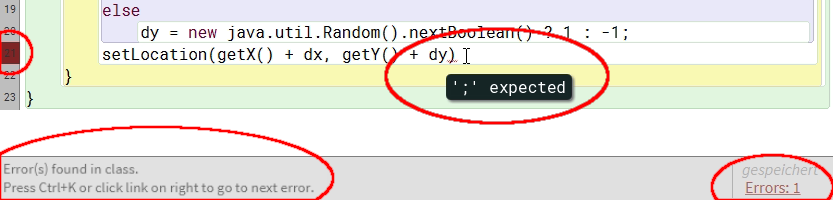
\includegraphics[width=4.5cm]{2.3.2.3/6.Uebungen/4-1.jpg}
    \end{figure}
    
    \barrow Auch hier muss man einfach nur die richtige Methode finden und gucken, was in der Signatur bezüglich des Parameters steht. Wir rufen die Methode \texttt{startsWith} mit dem Parameter \texttt{"Hallo"} am String auf und erhalten \texttt{true} oder \texttt{false}.
    
    \begin{figure}[ht]
	    \centering
	    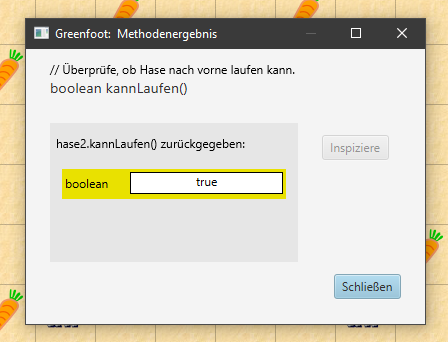
\includegraphics[width=4.5cm]{2.3.2.3/6.Uebungen/4-2.PNG}
    \end{figure}
	    
    \barrow String wird automatisch importiert, Random hingegen muss man manuell importieren. Anschließend erstellen wir ein neues Random-Objekt und rufen die Methode \texttt{nextInt} mit der Anzahl an Zahlen als Parameter an.
    
    \begin{figure}[ht]
	    \centering
	    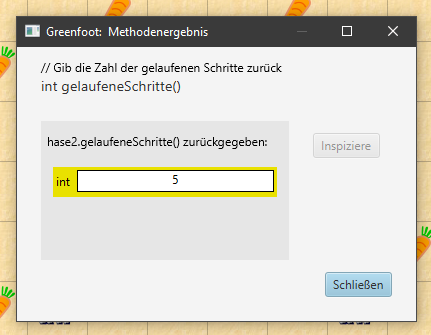
\includegraphics[height=2.5cm]{2.3.2.3/6.Uebungen/4-3.PNG}
	    \hspace{1cm}
	    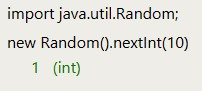
\includegraphics[height=2.5cm]{2.3.2.3/6.Uebungen/4-4.jpg}
    \end{figure}
    
    \newpage
    
    \barrow Dies funktioniert genauso wie gerade, nur mit der Methode \texttt{nextBoolean} und ohne Parameter.
    
    \begin{figure}[ht]
	    \centering
	    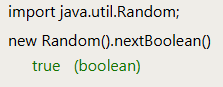
\includegraphics[width=4.5cm]{2.3.2.3/6.Uebungen/4-5.PNG}
    \end{figure}
    
    \vspace{2cm}
    
    \barrow Der sogenannte \glqq seed\grqq{} ist ein Startwert, von dem aus der Zufallsalgorithmus startet. Demnach sind die Zufallszahlen, welche wir benutzen, nicht wirklich zufällig. Wenn man immer mit demselben Seed starten würde, würden auch immer dieselben Zahlen herauskommen.
    
    Daher versucht man, einen Seed möglichst kompliziert und lang zu machen, jedoch soll es auch nicht zu viel Rechenleistung verbrauchen.\\
    
    Machen wir einen kleinen Test und erstellen zweimal mit demselben Seed Zufallszahlen und prüfen, ob dasselbe herauskommt.
    
    \begin{figure}[ht]
	    \centering
	    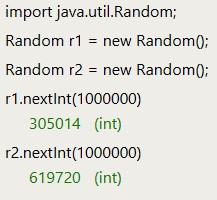
\includegraphics[height=4.5cm]{2.3.2.3/6.Uebungen/4-6.jpg}
	    \hspace{1cm}
	    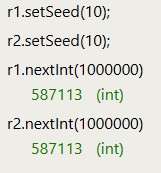
\includegraphics[height=4.5cm]{2.3.2.3/6.Uebungen/4-7.jpg}
    \end{figure}
    
    Wir sehen, dass zwei Random-Objekte mit automatischen Seeds verschiedene \glqq Zufallszahlen\grqq{} erzeugen. Wenn man dann jedoch beiden Objekten denselben Seed zuweist, erzeugen beide Objekte unabhängig voneinander dieselbe \glqq Zufallszahl\grqq{}. Und nein, das ist kein Zufall :), du kannst es ja auch mal ausprobieren.
    
    Aus diesem Grund kann der Seed bei Java als niedrigsten Wert $-9.223.372.036.854.775.808$\\
    und $9.223.372.036.854.775.807$ als höchsten Wert annehmen. Wie er genau errechnet wird, ist natürlich nicht öffentlich bekannt, sonst wäre es nicht mehr sicher.
\end{itemize}

\newpage

\subsection{Schleifen}

\begin{itemize}
    \item[\textbf{1.}]
    \begin{lstlisting}
void whileSchleife() {
    int zahl = 20;
    
    while (zahl != 0) {
        System.out.println(zahl);
        zahl--;
    }
}

void forSchleife() {
    for (int i = 20; i != 0; i--)   {
        System.out.println(i);
    }
}
    \end{lstlisting}
    \item[\textbf{2.}] Ich gehe davon aus, dass gemeint ist, dass alle geraden Zahlen über 0 ausgegeben werden sollen, denn sonst würde die Methode niemals enden.\\
    \begin{lstlisting}
void geradeZahlen_while(int n) {
    while (n >= 0) {
        if (n % 2 == 0) {
            System.out.println(n);
        }
        
        n--;
    }
}





void geradeZahlen_for(int n) {
    for (n = n; n >= 0; n--) {
        if (n % 2 == 0) {
            System.out.println(n);
        }
    }
}
    \end{lstlisting}
    Bei der for-Schleife hätte man auch eine extra Zählvariable ergänzen können, in diesem Fall habe ich aber \texttt{n} als Zählvariable benutzt.
    \item[\textbf{3.}] Ab sofort werde ich das Paket \texttt{java.util.Random}, falls \texttt{Random} benötigt ist, importieren, damit nicht bei jeder Zufallsgenerierung der \glqq etwas längliche \grqq{} Ausdruck benutzt werden muss. Stattdessen kann man ein Objekt erstellen und dies immer wieder verwenden. So auch hier:\\
    \begin{lstlisting}
import java.util.Random;

class Steuerung {
    int durchschnitt() {
        Random r = new Random();
        int summe = 0;

        for (int i = 0; i < 1000; i++) {
            summe += r.nextInt(11);
        }

        return summe / 1000;
    }

    void durchschnitte() {
        for (int i = 0; i < 25; i++) {
            System.out.println(durchschnitt());
        }
    }

    ...
}
    \end{lstlisting}
    
    Die zweite Methode zeigt 25 Ergebnisse der ersten Methode, um die Auswertung zu vereinfachen. Die Ausgabe zeigt ein ziemlich eindeutiges Ergebnis:
    
    \begin{figure}[ht]
	    \centering
	    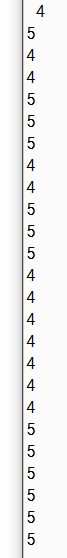
\includegraphics[height=14cm]{2.3.2.3/6.Uebungen/5-1.jpg}
    \end{figure}
    
    Anscheinend kommt jedes Mal 4 oder 5 heraus. Dieses Ergebnis beweist erneut, wie \glqq unzufällig\grqq{} die Zahlen des Zufallsalgorithmus sind.
    
    \newpage
    
    \item[\textbf{4.}]
    \begin{lstlisting}
int quadratzahlen(int n) {
    int summe = 0;
    
    for (int i = 1; Math.pow(i, 2) < n; i++) {
        System.out.println(Math.pow(i, 2));
        summe += Math.pow(i, 2);
    }
    
    return summe;
}
    \end{lstlisting}
    \item[\textbf{5.}] Es wird schwieriger...\\
    Angefangen habe ich damit, herauszufinden, wieviele Würfe man braucht, einmal einen Zweierpasch zu würfeln.\\
    \begin{lstlisting}
void zweierpasch() {
    Random r = new Random();
    int wuerfe = 0;
    
    int wuerfel1 = 0;
    int wuerfel2 = 0;
    
    while (wuerfel1 != 2 || wuerfel2 != 2) {
        wuerfel1 = r.nextInt(6) + 1;
        wuerfel2 = r.nextInt(6) + 1;
    
        wuerfe++;
    }
    
    System.out.println("Wuerfe: " + wuerfe);
}
    \end{lstlisting}
    
    \newpage
    
    Als nächstes wollen wir sicherstellen, dass der Wert aussagekräftig ist, also lassen wir den Prozess z.B. 1000 durchlaufen.\\
    \begin{lstlisting}
void zweierpasch() {
    Random r = new Random();
    int wuerfe = 0;
    
    for (int i = 0; i < 1000; i++) {
        int wuerfel1 = 0;
        int wuerfel2 = 0;
        
        while (wuerfel1 != 2 || wuerfel2 != 2) {
            wuerfel1 = r.nextInt(6) + 1;
            wuerfel2 = r.nextInt(6) + 1;

            wuerfe++;
        }
    }
    
    System.out.println("Wuerfe im Durchschnitt: " + wuerfe / 1000);
}
    \end{lstlisting}
    
    Der Wert bewegt sich immer circa um 36. Wenn wir diesen Wert mit dem Wert einer Einzelrunde vergleicht, fällt auf, dass die Einzelwerte starke Unterschiede aufweisen. Je öfter man es jedoch durchführt, desto genauer kann man eine Tendenz erkennen.
    
    Um zu überprüfen, ob das Programm richtig funktioniert, könnte man die 36 mathematisch als richtiges Ergebnis beweisen:
    
    Die Warscheinlichkeit eine 2 auf einem Würfel zu würfeln, beträgt logischerweise $\frac{1}{6}$. Also liegt die Warscheinlichkeit mit zwei Würfeln eine 2 zu würfeln bei $\frac{1}{6} * \frac{1}{6} = \frac{1}{36}$.
    
    Dieser Wert stimmt mit unserem überein. Mit einem von 36 Würfen wirft man im Durchschnitt einen Zweierpasch.
    
    \newpage
    
    \item[\textbf{6.}] Ich gebe zwei Beispiele für Endlosschleifen, denn es gibt viele Beispiele. Viel Spaß beim Kreieren weiterer Endlosschleifen.\\
    \begin{lstlisting}
while (true) {
    ...
}
    \end{lstlisting}
    \begin{lstlisting}
for (int i = 0; i >= 0; i++) {
    testMethode();
}
    \end{lstlisting}
\end{itemize}

\end{document}